% Preamble
% Compile with XeLateX

\documentclass[11 pt,oneside,a4paper,titlepage]{article}
\usepackage{preamble}
\graphicspath{{PIC/}}
\usepackage{xcolor}
\definecolor{mitred}{RGB}{163,31,52}
\definecolor{mitgray}{RGB}{119,119,119}
\definecolor{Magenta}{RGB}{255, 0, 255}
%%%%%%%%%%%%%%%%%%%%%%%%%%%%%%%%%%%%%%%%%%%%%%%%%%%%%%%%%%%%%%%%%%%%%%%%%%%%%%%%%%%%%%
\begin{document}

\sidebar{sideBarColor!20}
\simpleheader{titleBackColor!60}{Md}{Al-Mamun}{}{white}

% Start Minipages
\vspace*{3.49cm}% start 8 cm from the top of the page}
    \adjustbox{valign=t}{\begin{minipage}{7.3cm} % large 7.4 cm from the top
    \vspace*{1.2cm} % text starts 1cm under the top of the minipage
            
        % Picture
        \begin{center}
        \begin{tikzpicture}
            \node[
            circle,
            minimum size=\cvPictureWidth,
            path picture={
            \node at (path picture bounding box.center){
             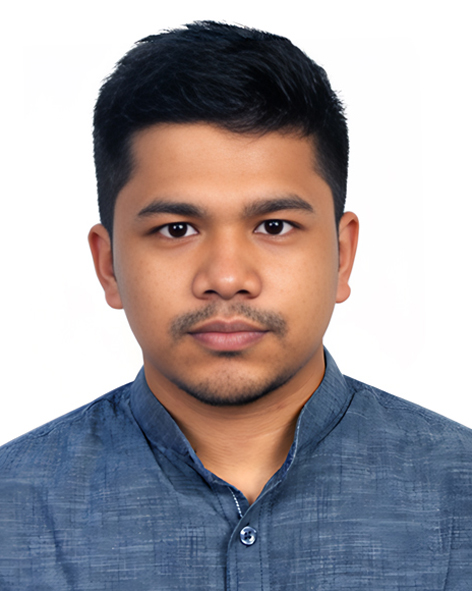
\includegraphics[width=\cvPictureWidth]{PIC/3R=1.jpg}
             };
             }]
            {};
        \end{tikzpicture}
        \end{center}

        %%%%%%%%%%%%%%%%%%%%%%%%%%%%%%%%%%%%%%%%%%%%%%%%%%%%
        % Profile section
        \ruleline{\textbf{\textcolor{mitred}{About me}}}
        %\lipsum[150] %
       I am Proficient in various operating systems such as Windows, Linux, and MacOS. Strong knowledge of virtualization technologies such as VMware and Hyper-V. Passionate about emerging technologies and dedicated to staying up-to-date with the latest industry trends. I am highly proficient in SQL, Python, and data visualization tools such as Tableau, and I am skilled at communicating complex information to both technical and non-technical audiences. I am passionate about using data to drive business success, and am constantly seeking new ways to improve my skills and stay ahead of the curve in this dynamic field.
        %%%%%%%%%%%%%%%%%%%%%%%%%%%%%%%%%%%%%%%%%%%%%%%%%%%
        % Contact Section
        \ruleline{\textbf{\textcolor{mitred}{Contact}}}
        \begin{tikzpicture}[every node/.style={inner sep=0pt, outer sep=0pt}]
        \matrix [
        column 1/.style={anchor=center,contactIcon},
        column 2/.style={anchor=west,align=left,contactIcon},
        column sep=5pt,
        row sep=5pt] (contact) {
        \node{\faMale};
         & \node{Born on 01/08/1998, Age 25};\\
        \node{\faEnvelope}; 
         & \node{\href{mailto:md.4lmamun@gmail.com}{md.4lmamun@gmail.com}};\\
        \node{\faPhone}; 
         & \node{+880 1794-094268};\\ 
        \node{\faMapMarker}; 
        & \node{Nobabgonj, Lalbagh, Dhaka-1211};\\
        \node{\faLinkedinSquare}; 
        & \node{\href{https://www.linkedin.com/in/itsmealamin/}{Md Al-Mamun}};\\
        \node{\aiResearchGateSquare}; 
        & \node{\href{https://www.researchgate.net/profile/Md-Al-Mamun-25}{Research Gate: Md Al-Mamun}};\\
        \node{\faGithub}; 
        & \node{\href{https://github.com/TomBombadi1}{Github: Al-Amin}};\\
        };
        \end{tikzpicture} 
        
        %%%%%%%%%%%%%%%%%%%%%%%%%%%%%%%%%%%%%%%%%%%%%%%%%%%
        \ruleline{\textbf{\textcolor{mitred}{Languages}}}
        \begin{tikzpicture}[every node/.style={inner sep=0pt, outer sep=0pt}]
        \matrix [
        column 1/.style={anchor=center,contactIcon},
        column 2/.style={anchor=west,align=left,contactIcon},
        column sep=5pt,
        row sep=5pt] (contact) {
        \node{\flag{Bangladesh.png}};
        & \node{Bengali - Native Language};\\
        \node{\flag{England.png}};
        & \node{English - Professional Language};\\
        };
        \end{tikzpicture} 
        \vspace*{0.5cm}
        %%%%%%%%%%%%%%%%%%%%%%%%%%%%%%%%%%%%%%%%%%%%%%%%%%%%%
        % QR Code
        \scriptsize
        \begin{center}
            \quad
            \qrcode[height=3.5cm]{
               https://www.hackerrank.com/mac4br3?hr_r=1/} \\
            \vspace*{0.5cm}
        \end{center}
        
    \end{minipage}} %
    \hfill 
%%%%%%%%%%%%%%%%%%%%%%%%%%%%%%%%%%%%%%%%%%%%%%%%%%%%%%%%%
%%%%% MAIN SECTION %%%%%%%%%%%%%%%%%%%%
    \adjustbox{valign=t}{\begin{minipage}{11.3cm}
        \vspace*{1cm}
        \section*{\textcolor{mitred}{{\faGraduationCap} EDUCATION}}

        \MySection{\textcolor{mitgray}{2018-2022}}{wub.png}{B.Sc}{World University of Bangladesh}{Dhaka, Bangladesh}{Computer Science \& Engineering}{During their undergraduate years, I demonstrated exceptional aptitude in various areas of CSE, including programming, algorithms, software development, and data structures. My was consistently excelled in my coursework, displaying a deep understanding of fundamental concepts and their practical applications. Apart from academic achievements, I was actively engaged in extracurricular activities related to CSE. My participated in coding competitions, hackathons, and technology-oriented clubs, help me to honing my problem-solving skills and collaborative abilities.  \\\textbf{C.G.P.A: 2.87/4.00 }}
            
        \vspace*{0.22cm}
            
        \MySection{\textcolor{mitgray}{2015-2017}}{NISC.png}{H.S.C}{Nabakumar Institution \& Dr. Shahidullah College}{Dhaka, Bangladesh}{Science}{
Firstly, science helps our understanding of the world around us. Everything we know about the universe, from how trees reproduce to what an atom is made up of, is the result of scientific research and experiment. Human progress throughout history has largely rested on advances in science.\\\textbf{G.P.A: 3.29/5.00}}
                
        %%%%%%%%%%%%%%%%%%%%%%%%%%%%%%%%%%%%%%%%%%%%%%%%%%%
        % Work Experience
        \section*{\textcolor{mitred}{{\faSuitcase} WORK \& TRAINING EXPERIENCE}}
            
        \MySectionNoPic{\textcolor{mitgray}{2018-2019}}{Asst. Supervisor}{Dhaka, Bangladesh}{\textbf{China Harbour Engineering Company}}{It was a project under the Bangladesh govt. Here my technical work was to Measured and marked property lines and key topographic features. Supervised survey projects measuring volume capacity of landfills and containment ponds.}  
            
        \vspace*{0.22cm}
            
        \MySectionNoPic{\textcolor{mitgray}{2020-2021}}{Account Officer}{Dhanmondi, Dhaka}{\textbf{The Buffet show Restaurent}}{Here my technical work was to Developed and executed marketing programs and general business solutions resulting in increased
company exposure, customer traffic and elevated sales numbers. Developed technical and non-technical marketing
presentations, public relations campaigns, articles and newsletters.}  

            \vspace*{0.22cm}
            
        \MySectionNoPic{\textcolor{mitgray}{2023}}{Big Data Analytic \& Data Science}{Dhaka}{\textbf{BASIS-Skills For Employment Investment Program}}{Here I experience Analytical Expertise on Data analysis and Data manipulation.I have learn Data Visualization and Feature Engineering.And how to train Data by using ML technique for prediction and Other Services.}  
        \vspace*{0.6cm}
%%%%%%%%%%%%%%%%%%%% 
%%%%%%%%%%%%%%%%%%%%%%%%%%%%%%%%%%%%%%%%%%%%%%%%%%%
        %Publications
        \section*{\textcolor{mitred}{{\aiOBP} PUBLICATIONS/PROJECT}}
            
        \publication{Thesis}{2022}{HMalware Detection using Machine Learning Model}{Md Al-Mamun, Md Redwan, Tamanna Zaman Tammi}{World University of Bangladesh}{372763590}
            
        \vspace*{0.22cm}
             
        \publication{Journal}{on-going}{Informstion Security on Big Data}{Md Al-Mamun}{Personal}{}
            
        \vspace*{0.22cm}
            
        % \publication{Conference Proceedings}{1724}{How I lost my ship and how to get it back}{Jack Sparrow}{Conference in Tortuga}{10.5220/doidoidoi}
    %%%%%%%%%%%%%%%%%%%%%%%%%%%%%%%%%%%%%%%%%%%%%%%%%%%
    \end{minipage}} %

% Second Page
\newpage

\sidebar{sideBarColor!20}
\newpageheader{mitgray}{Md}{Al-Mamun}{Python Programmer 
 \faLightbulbO \hspace{1mm} Data Analyst}{white}

% %%%%%%%%%%%%%%%%%%%%%%%%%%%%%%%%%% SIDEBAR %%%%%%%%%%%%%%%%%%%
\adjustbox{valign=t}{
\begin{minipage}{7.3cm} 
\vspace*{0.4cm} % text starts 0.4cm under the top the header

%%%%%%%%%%%5%%%%%%%%%%%%%%%%
% Skill and Strengths 
    \ruleline{\textbf{\textcolor{mitred}{{Soft Skills and Strengths}}}}
    \vspace*{-0.5cm}
    \begin{center}
       \cvtag{Curiosity}\cvtag{Flexibility}\cvtag{Self Confidence}\cvtag{Adaptability} \cvtag{Eye for Details}\cvtag{Problem Solving}\cvtag{Team Working}\cvtag{Love Learning New Things}\cvtag{Good Communication}\cvtag{Diplomacy}\cvtag{Good Listener}\cvtag{Patience}
    \end{center}

 \vspace*{0.6cm}
%%%%%%%%%%%%%%%%%%%%%%%%%%%%%%%%%%%%%%%%%%%%%%%%%%%%
    % Professional Skills 
    \ruleline{\textbf{\textcolor{mitred}{{Professional Skills}}}}
    \begin{center}
       \cvtag{Python}\cvtag{R programming Language}\cvtag{MySQL/ PostgreSQL/OracleDBA}\cvtag{Bash Scripting}\cvtag{Web Scraping}\cvtag{Machine Learning}\cvtag{Artificial Intelligence}\cvtag{Statistical Programming}\cvtag{Rust}\cvtag{C++}\cvtag{LaTex}\cvtag{Pandas/Numpy/Seaborn}\cvtag{Keras/ Scikit-learn}\cvtag{Tensorflow}\cvtag{Google Data studio/Power BI / Tableau}
    \end{center}
%%%%%%%%%%%%%%%%%%%%%%%%%%%%%%%%%%%%%%%%%%%%%%%%%%%%%%%%%%%%
    % Other Interests
    \ruleline{\textbf{\textcolor{mitred}{Interests}}}
    \small
    \begin{multicols}{2}
        \begin{itemize} 
            \item  Guitar \flag{Guitar.png}
            \item  Chess \flag{Chess.png}
            \item  Travels \flag{Travels.png}
            \item  Movies \flag{movie2.png}
            \item  Books \flag{Books.png}
            \item  Food  \flag{food.png}
    \end{itemize}
    \end{multicols}

     %%%%%%%%%%%%%%%%%%%%%%%%%%%%%%%%%%%%%%%%%%%%%%%%%%%%%
        % QR Code
        \ruleline{\textbf{\textcolor{mitred}{Download My CV}}}
        \scriptsize
        \centering
        Download my CV via the QR below \aiOverleaf.
        \begin{center}
            \quad
            \qrcode[height=3cm]{
                https://github.com/TomBombadi1/Latex-CV-Template.git} \\
            \vspace*{0.5cm}
        \end{center}

\end{minipage}
}%
\hfill
%%%%%%%%%%%%%%%%%%%%%%%%%%%%%%%%%%% MAIN %%%%%%%%%%%%%%%%%%%%%%%%%
\adjustbox{valign=t}{%
\begin{minipage}{11.3cm}
    \vspace*{0.4cm}
    %%%%%%%%%%%%%%%%%%%%%%%%%%%%%%%%%%%%%%%%%%%%%%%%%%%
    % Peer Reviews
    \section*{\textcolor{mitred}{{\faBook} ACADEMIC PEER REVIEWS}}
    \footnotesize I did academic peer review for the following journals: 
    \begin{itemize}
        \footnotesize
         \item{\textbf{Malware Detection using Machine Learning Model}, March 12, 2022;}
          \footnotesize
         \item{\textbf{Human emotion classification with CNN LSTM model from
        speech}, March 12, 2022;}
     \end{itemize}
        
    %%%%%%%%%%%%%%%%%%%%%%%%%%%%%%%%%%%%%%%%%%%%%%%%%%%
    % Information Technology Skills
    \section*{\textcolor{mitred}{{\faDesktop} INFORMATION TECHNOLOGY SKILLS}}
    
    \ITCcompetence{Data Analysis}{
    \textbf{Jupyter Notebook}: \textit{Higly Specialized}\\
    \textbf{Matlab}: \textit{Intermediate}\\
    \textbf{Tableau}: \textit{Intermediate}\\
    }

    \ITCcompetence{Operating System}{
    \textbf{Windows}: \textit{Higly Specialized}\\
    \textbf{MacOS}: \textit{Intermediate}\\
    \textbf{Linux}: \textit{Higly Specialized}\\
    \textbf{Linux Server}: \textit{Intermediate}
    }
    
    % \vspace*{0.22cm}

    % \ITCcompetence{Modeling and Simulation}{
    % \textbf{Simulink} : \textit{Intermediate}  \\
    % \textbf{LTSpice}: \textit{Intermediate}
    % }
    
    % \vspace*{0.22cm}

    % \ITCcompetence{Audio Processing}{
    % \textbf{Reaper} : \textit{Advanced}  \\
    % }

    \vspace*{0.22cm}

    \ITCcompetence{Office Automation}{
    \textbf{MS Office (Excel, Word, PowerPoint)}: \textit{Higly Specialized}\\
    \textbf{\LaTeX}: \textit{Advanced}\\
    \textbf{Prezi}: \textit{Intermediate}\\
    }
    
    %%%%%%%%%%%%%%%%%%%%%%%%%%%%%%%%%%%%%%%%%%%%%%%%%%%
    % Programming Languages
    \section*{\textcolor{mitred}{{\faCode} PROGRAMMING LANGUAGES}}
    \vspace*{-0.5cm}
    \begin{multicols}{2}    
    \begin{itemize}
    \footnotesize
        \item \textbf{Python}: Advanced
        \item \textbf{Bash Script}: Intermediate
        \item \textbf{SQL}: Intermediate
        % \item \textbf{C/C++}: Intermediate
        \item \textbf{R}: Intermediate 
        \item \textbf{HTML / CSS}: Advanced
        \item \textbf{JavaScript}: Intermediate
        \item \textbf{Rust}: Basic
        \item \textbf{Matlab}: Basic
        \item \textbf{Go}: Basic
        \item \textbf{Apache Spark}: Basic
        \item \textbf{Dart/Flutter}: Intermediate 
        \item[\vspace{\fill}]
    \end{itemize}
    \end{multicols}
    
    %%%%%%%%%%%%%%%%%%%%%%%%%%%%%%%%%%%%%%%%%%%%%%%%%%%
    % Certificates
    \section*{\textcolor{mitred}{{\faCertificate} CERTIFICATES}}
    
    \adjustbox{valign=t}{\begin{minipage}{2cm}
    \begin{center}
        
\includegraphics[width=1.2cm]{IBM.png}
    \end{center}
    \end{minipage}}
    \hfill \vline \hfill
    \adjustbox{valign=t}{\begin{minipage}{9cm}
        \begin{itemize}
            \scriptsize 
            \item Python for Data Science, AI \& Development (\textbf{\textit{Coursera, 2022}})
            \item Cybersecurity Compliance Framework \& System Administration (\textbf{\textit{Coursera, 2022}})
        \end{itemize}
    \end{minipage}}
    
    \vspace*{0.2cm}
    
    \adjustbox{valign=t}{\begin{minipage}{2cm}
    \begin{center}
        
\includegraphics[width=1.2cm]{google.png}
    \end{center}
    \end{minipage}}
    \hfill \vline \hfill
    \adjustbox{valign=t}{\begin{minipage}{9cm}
        \begin{itemize}
            \scriptsize 
            \item Crash Course on Python (\textbf{Coursera 2020})
            \item Google Data Analytics Professional Certificate (\textbf{Google 2022})
            \item Artificial Intelligence Foundations: Machine Learning (\textbf{Linkedin 2021})
        \end{itemize}
    \end{minipage}}

     \vspace*{0.2cm}
    
    \adjustbox{valign=t}{\begin{minipage}{2cm}
    \begin{center}
        
\includegraphics[width=1.2cm]{cit.png}
    \end{center}
    \end{minipage}}
    \hfill \vline \hfill
    \adjustbox{valign=t}{\begin{minipage}{9cm}
        \begin{itemize}
            \scriptsize 
            \item Certified Ethical Hacking - \textbf{CreativeIT institute -2021}
            \item Python for Machine Learning -\textbf{CreativeIT institute -2019} 
        \end{itemize}
    \end{minipage}}
    
    \vspace*{0.2cm}

    \adjustbox{valign=t}{\begin{minipage}{2cm}
    \begin{center}
        \includegraphics[width=1.2cm]{th-2688257842.jpeg}
    \end{center}
    \end{minipage}}
    \hfill \vline \hfill
    \adjustbox{valign=t}{\begin{minipage}{9cm}
        \begin{itemize}
            \scriptsize 
            \item Data Science \& Big Data Analysis -\textbf{BASIS/SEIP -2023}
        \end{itemize}
    \end{minipage}}
    
    \vspace*{0.2cm}
    
\end{minipage}}


\end{document}
